%===============================================================================
% LaTeX sjabloon voor de bachelorproef toegepaste informatica aan HOGENT
% Meer info op https://github.com/HoGentTIN/bachproef-latex-sjabloon
%===============================================================================

\documentclass{bachproef-tin}

\usepackage{hogent-thesis-titlepage} % Titelpagina conform aan HOGENT huisstijl

%%---------- Documenteigenschappen ---------------------------------------------
% TODO: Vul dit aan met je eigen info:

% De titel van het rapport/bachelorproef
\title{Titel}

% Je eigen naam
\author{Angelo Carly}

% De naam van je promotor (lector van de opleiding)
\promotor{Jan Janssens}

% De naam van je co-promotor. Als je promotor ook je opdrachtgever is en je
% dus ook inhoudelijk begeleidt (en enkel dan!), mag je dit leeg laten.
\copromotor{Wannes Van Dorpe}

% Indien je bachelorproef in opdracht van/in samenwerking met een bedrijf of
% externe organisatie geschreven is, geef je hier de naam. Zoniet laat je dit
% zoals het is.
\instelling{---}

% Academiejaar
\academiejaar{2019-2020}

% Examenperiode
%  - 1e semester = 1e examenperiode => 1
%  - 2e semester = 2e examenperiode => 2
%  - tweede zit  = 3e examenperiode => 3
\examenperiode{2}

%===============================================================================
% Inhoud document
%===============================================================================

\begin{document}

%---------- Taalselectie -------------------------------------------------------
% Als je je bachelorproef in het Engels schrijft, haal dan onderstaande regel
% uit commentaar. Let op: de tekst op de voorkaft blijft in het Nederlands, en
% dat is ook de bedoeling!

%\selectlanguage{english}

%---------- Titelblad ----------------------------------------------------------
\inserttitlepage

%---------- Samenvatting, voorwoord --------------------------------------------
\usechapterimagefalse
%%=============================================================================
%% Voorwoord
%%=============================================================================

\chapter*{Woord vooraf}
\label{ch:voorwoord}

%% TODO:
%% Het voorwoord is het enige deel van de bachelorproef waar je vanuit je
%% eigen standpunt (``ik-vorm'') mag schrijven. Je kan hier bv. motiveren
%% waarom jij het onderwerp wil bespreken.
%% Vergeet ook niet te bedanken wie je geholpen/gesteund/... heeft


%%=============================================================================
%% Samenvatting
%%=============================================================================

% TODO: De "abstract" of samenvatting is een kernachtige (~ 1 blz. voor een
% thesis) synthese van het document.
%
% Deze aspecten moeten zeker aan bod komen:
% - Context: waarom is dit werk belangrijk?
% - Nood: waarom moest dit onderzocht worden?
% - Taak: wat heb je precies gedaan?
% - Object: wat staat in dit document geschreven?
% - Resultaat: wat was het resultaat?
% - Conclusie: wat is/zijn de belangrijkste conclusie(s)?
% - Perspectief: blijven er nog vragen open die in de toekomst nog kunnen
%    onderzocht worden? Wat is een mogelijk vervolg voor jouw onderzoek?
%
% LET OP! Een samenvatting is GEEN voorwoord!

%%---------- Nederlandse samenvatting -----------------------------------------
%
% TODO: Als je je bachelorproef in het Engels schrijft, moet je eerst een
% Nederlandse samenvatting invoegen. Haal daarvoor onderstaande code uit
% commentaar.
% Wie zijn bachelorproef in het Nederlands schrijft, kan dit negeren, de inhoud
% wordt niet in het document ingevoegd.

\IfLanguageName{english}{%
\selectlanguage{dutch}
\chapter*{Samenvatting}
%tekst
\selectlanguage{english}
}{}

%%---------- Samenvatting -----------------------------------------------------
% De samenvatting in de hoofdtaal van het document

\chapter*{\IfLanguageName{dutch}{Samenvatting}{Abstract}}

teksts


%---------- Inhoudstafel -------------------------------------------------------
\pagestyle{empty} % Geen hoofding
\tableofcontents  % Voeg de inhoudstafel toe
\cleardoublepage  % Zorg dat volgende hoofstuk op een oneven pagina begint
\pagestyle{fancy} % Zet hoofding opnieuw aan

%---------- Lijst figuren, afkortingen, ... ------------------------------------

% Indien gewenst kan je hier een lijst van figuren/tabellen opgeven. Geef in
% dat geval je figuren/tabellen altijd een korte beschrijving:
%
%  \caption[korte beschrijving]{uitgebreide beschrijving}
%
% De korte beschrijving wordt gebruikt voor deze lijst, de uitgebreide staat bij
% de figuur of tabel zelf.

\listoffigures
\listoftables

% Als je een lijst van afkortingen of termen wil toevoegen, dan hoort die
% hier thuis. Gebruik bijvoorbeeld de ``glossaries'' package.
% https://www.overleaf.com/learn/latex/Glossaries

%---------- Kern ---------------------------------------------------------------

% De eerste hoofdstukken van een bachelorproef zijn meestal een inleiding op
% het onderwerp, literatuurstudie en verantwoording methodologie.
% Aarzel niet om een meer beschrijvende titel aan deze hoofstukken te geven of
% om bijvoorbeeld de inleiding en/of stand van zaken over meerdere hoofdstukken
% te verspreiden!

%%=============================================================================
%% Inleiding
%%=============================================================================

\chapter{\IfLanguageName{dutch}{Inleiding}{Introduction}}
\label{ch:inleiding}

%De inleiding moet de lezer net genoeg informatie verschaffen om het onderwerp te begrijpen en in te zien waarom de onderzoeksvraag de moeite waard is om te onderzoeken. In de inleiding ga je literatuurverwijzingen beperken, zodat de tekst vlot leesbaar blijft. Je kan de inleiding verder onderverdelen in secties als dit de tekst verduidelijkt. Zaken die aan bod kunnen komen in de inleiding~\autocite{Pollefliet2011}:

%\begin{itemize}
  %\item context, achtergrond
  %\item afbakenen van het onderwerp
  %\item verantwoording van het onderwerp, methodologie
  %\item probleemstelling
  %\item onderzoeksdoelstelling
  %\item onderzoeksvraag
  %\item \ldots
%\end{itemize}

%Vandaag de dag heeft UGent enkele problemen met de toegangscontrole van hun parking. Het huidige systeem met tokens is een oude technologie en is aan vernieuwing toe.

\section{\IfLanguageName{dutch}{Probleemstelling}{Problem Statement}}
\label{sec:probleemstelling}

%Uit je probleemstelling moet duidelijk zijn dat je onderzoek een meerwaarde heeft voor een concrete doelgroep. De doelgroep moet goed gedefinieerd en afgelijnd zijn. Doelgroepen als ``bedrijven,'' ``KMO's,'' systeembeheerders, enz.~zijn nog te vaag. Als je een lijstje kan maken van de personen/organisaties die een meerwaarde zullen vinden in deze bachelorproef (dit is eigenlijk je steekproefkader), dan is dat een indicatie dat de doelgroep goed gedefinieerd is. Dit kan een enkel bedrijf zijn of zelfs één persoon (je co-promotor/opdrachtgever).

Vandaag de dag kampt UGent met problemen omtrent hun toegangssysteem van hun parking aan de campus Coupure en campus Sterre. Het huidige systeem dat gebruikt maakt van tokens is niet efficiënt en zorgt voor veel extra werk. Dit is werk zoals:
\begin{itemize}
	\item De tokens moeten telkens afgehaald worden aan het onthaal om de campussen te kunnen verlaten.
	\item De tokenslikkers moeten regelmatig geleegd worden indien de tokenslikkers vol zijn.
	\item De tokens zijn relatief duur om bij te maken.
	\item De tokens worden snel kwijtgeraakt.
\end{itemize}
Door deze problemen overweegt UGent om op deze locaties over te stappen naar een beter systeem dat milieubewust is, beperkt in kostprijs is, en een goed gebruiksgemak heeft. 

Hierop biedt VaDo Solutions een innovatief systeem aan dat gebruik maakt van nummerplaatdetectie. Deze zou gebruik maken van een Raspberry PI in combinatie met een open-source library genaamd OpenALPR. Welke al reeds bevestigd zijn dat ze goede resultaten kunnen opleveren \autocite{figuerola2016automated}. Maar of deze resultaten ook haalbaar zijn op UGent kan hiermee niet bevestigd worden. Dit zal dit onderzoek nagaan.

Vervolgens heerst er ook nog enkele onduidelijkheid over hoe de GDPR inspeelt op een dergelijk systeem en welke maatregelingen hierrond getroffen moeten worden.

\section{\IfLanguageName{dutch}{Onderzoeksvraag}{Research question}}
\label{sec:onderzoeksvraag}

%Wees zo concreet mogelijk bij het formuleren van je onderzoeksvraag. Een onderzoeksvraag is trouwens iets waar nog niemand op dit moment een antwoord heeft (voor zover je kan nagaan). Het opzoeken van bestaande informatie (bv. ``welke tools bestaan er voor deze toepassing?'') is dus geen onderzoeksvraag. Je kan de onderzoeksvraag verder specifiëren in deelvragen. Bv.~als je onderzoek gaat over performantiemetingen, dan 
Dit onderzoek zal nagaan in hoeverre het mogelijk is nummerplaatdetectie op te stellen op de Campus Coupure en Campus Sterre van UGent. Hiervoor wordt er bekeken in welke mate de GDPR invloed heeft op nummerplaatdetectie. Daarnaast zullen er maatregelingen opgesteld worden om een nauwkeurige detectie te verkrijgen, waarop er vervolgens een testopstelling gemaakt wordt om na te gaan of een dit wel degelijk mogelijk is op UGent.

Zo bekomen we volgende drie onderzoeksvragen:
\begin{itemize}
	\item Is nummerplaatdetectie een haalbare techniek omtrent GDPR?
	\item Welke maatregelingen moeten er genomen worden om succesvol nummerplaatdetectie te implementeren?
	\item Kan men nummerplaatdetectie succesvol uitvoeren met een Raspberry PI op de campus Coupure en Sterre van UGent?
\end{itemize}

Deze vragen zullen doorheen dit onderzoek beantwoord worden.

\section{\IfLanguageName{dutch}{Onderzoeksdoelstelling}{Research objective}}
\label{sec:onderzoeksdoelstelling}

%Wat is het beoogde resultaat van je bachelorproef? Wat zijn de criteria voor succes? Beschrijf die zo concreet mogelijk. Gaat het bv. om een proof-of-concept, een prototype, een verslag met aanbevelingen, een vergelijkende studie, enz.

Dit onderzoek heeft tot doel om een correcte voorstelling te geven over hoe nauwkeurig nummerplaatdetectie met een Raspberry Pi en OpenALPR uitgevoerd kan worden op UGent. Dit zal gedaan worden door een prototype hiervan op te stellen en uit te testen aan de uitgangen van UGent Campus Sterre en Campus Coupure. Door de resultaten van dit onderzoek zal VaDo-Solutions kunnen beslissen of dit wel of niet de gewenste technologie is die zij willen gebruiken.

Vervolgens wordt er verwacht dat een duidelijk overzicht gegeven wordt van maatregelingen die getroffen kunnen worden om een dergelijk systeem te implementeren. Deze zullen zijn op vlak van hardware- en software-instellingen zowel als fysieke variabelen zoals locatie en richting. Zo kan een installateur op een vlotte manier inzicht verkrijgen welke factoren een grote bijdrage leveren aan een nauwkeurig ANPR-systeem.

Ten laatste is het de bedoeling om een bondige uitleg te hebben op welke vlakken de GDPR invloed heeft op dit soort camerasysteem. Hiermee kan een ontwikkelaar weten aan welke voorwaarden zijn opstelling moet voldoen zodat hij geen risico loopt op het overtreden van deze wetgevingen.

\section{\IfLanguageName{dutch}{Opzet van deze bachelorproef}{Structure of this bachelor thesis}}
\label{sec:opzet-bachelorproef}

% Het is gebruikelijk aan het einde van de inleiding een overzicht te
% geven van de opbouw van de rest van de tekst. Deze sectie bevat al een aanzet
% die je kan aanvullen/aanpassen in functie van je eigen tekst.

De rest van deze bachelorproef is als volgt opgebouwd:

In Hoofdstuk~\ref{ch:stand-van-zaken} wordt een overzicht gegeven van de stand van zaken binnen het onderzoeksdomein, op basis van een literatuurstudie.

In Hoofdstuk~\ref{ch:methodologie} wordt de methodologie toegelicht en worden de gebruikte onderzoekstechnieken besproken om een antwoord te kunnen formuleren op de onderzoeksvragen.

In Hoofdstuk~\ref{ch:wetgeving-nummerplaatdetectie} wordt er nagegaan waarop er gelet moet worden bij het implementeren van nummerplaatdetectie als toegangssysteem op vlak van privacywetgevingen.

In Hoofdstuk~\ref{ch:maatregelenanpr} wordt er nagegaan welke maatregelingen er genomen moeten worden om een zo performant mogelijke implementatie van nummerplaatdetectie te maken.

In Hoofdstuk~\ref{ch:praktischeUitvoering} wordt een steekproef uitgevoerd aan de hand van de vooropgestelde maatregelingen aan de campus Sterre en Coupure van UGent. Hieruit zal blijken of nummerplaatdetectie met een Raspberry PI wel degelijk mogelijk is op deze locatie.

In Hoofdstuk~\ref{ch:conclusie}, tenslotte, wordt de conclusie gegeven en een antwoord geformuleerd op de onderzoeksvragen. Daarbij wordt ook een aanzet gegeven voor toekomstig onderzoek binnen dit domein.
\chapter{\IfLanguageName{dutch}{Stand van zaken}{State of the art}}
\label{ch:stand-van-zaken}

% Tip: Begin elk hoofdstuk met een paragraaf inleiding die beschrijft hoe
% dit hoofdstuk past binnen het geheel van de bachelorproef. Geef in het
% bijzonder aan wat de link is met het vorige en volgende hoofdstuk.

% Pas na deze inleidende paragraaf komt de eerste sectiehoofding.

%Dit hoofdstuk bevat je literatuurstudie. De inhoud gaat verder op de inleiding, maar zal het onderwerp van de bachelorproef *diepgaand* uitspitten. De bedoeling is dat de lezer na lezing van dit hoofdstuk helemaal op de hoogte is van de huidige stand van zaken (state-of-the-art) in het onderzoeksdomein. Iemand die niet vertrouwd is met het onderwerp, weet nu voldoende om de rest van het verhaal te kunnen volgen, zonder dat die er nog andere informatie moet over opzoeken \autocite{Pollefliet2011}.

%Je verwijst bij elke bewering die je doet, vakterm die je introduceert, enz. naar je bronnen. In \LaTeX{} kan dat met het commando \texttt{$\backslash${textcite\{\}}} of \texttt{$\backslash${autocite\{\}}}. Als argument van het commando geef je de ``sleutel'' van een ``record'' in een bibliografische databank in het Bib\LaTeX{}-formaat (een tekstbestand). Als je expliciet naar de auteur verwijst in de zin, gebruik je \texttt{$\backslash${}textcite\{\}}.
%Soms wil je de auteur niet expliciet vernoemen, dan gebruik je \texttt{$\backslash${}autocite\{\}}. In de volgende paragraaf een voorbeeld van elk.

%\textcite{Knuth1998} schreef een van de standaardwerken over sorteer- en zoekalgoritmen. Experten zijn het erover eens dat cloud computing een interessante opportuniteit vormen, zowel voor gebruikers als voor dienstverleners op vlak van informatietechnologie~\autocite{Creeger2009}.

In dit hoofdstuk zal uitgelegd worden wat de huidige stand van zaken is van toegangssystemen bij de parking van UGent en welke andere technologieën hiervoor hedendaags gebruikt worden.
Verder wordt er besproken wat de GDPR inhoudt en waar deze op slaat. Ten laatste wordt er bekeken wat de voorgestelde hardware betreft voor dit onderzoek.

\section{Huidige situatie UGent}
% Huidige situatie UGent

Het huidige toegangssysteem aan UGent op de beschreven locaties is een systeem op basis van tokens. Een bezoeker rijdt de parking op zonder enige checks. Vervolgens bezoekt hij de campus en vraagt een token om de campus te verlaten. Ten laatste rijdt hij zijn wagen naar de slagboom en geeft zijn token in de gepaste tokenslikker.
Op de campus Sterre zijn er 3 ingangen en 2 uitgangen, op de campus Landbouw is dit gelijkaardig met 3 ingangen en 2 uitgangen.

\subsection{Technologieën in gebruik}
Meerdere toegangssystemen zijn vandaag de dag al in gebruik aan de campussen Landbouw en Sterre. Voor de toegang van personeel, studenten en bezoekers.

\subsubsection{Tokens}

%Hoe werken de tokens
Tokens worden aan alle uitgangen van de campussen gebruikt om de parking te verlaten.
Tokens worden hoofdzakelijk gebruikt om de parking te verlaten, alle uitgangen beschikken over een tokenslikker. Op deze manier kunnen studenten of bezoekers de campus verlaten nadat zij een token gaan afhalen op het onthaal.

%Nadelen van tokens
De tokens zelf vallen momenteel niet in goede aard omdat deze enkele nadelen met zich meebrengen:
\begin{itemize}
	\item De tokens worden veel misbruikt op faciliteiten buiten UGent zoals automaten, carwashes en meer.
	\item De tokens zelf kunnen makkelijk verloren geraken, wat niet milieubewust is.
	\item De tokens zelf redelijk duur aan een kost van 1,5 euro per stuk.
\end{itemize}

Deze punten geven aan dat tokens niet de gewenste oplossing zijn voor de campussen van UGent. Dit is te merken aan de hoofduitgang van de Campus Landbouw waar de uitgang vrij is om door te laten omdat de slikkers te veel werk met zich meebrengen.

\begin{figure}[h!]
	\centering
	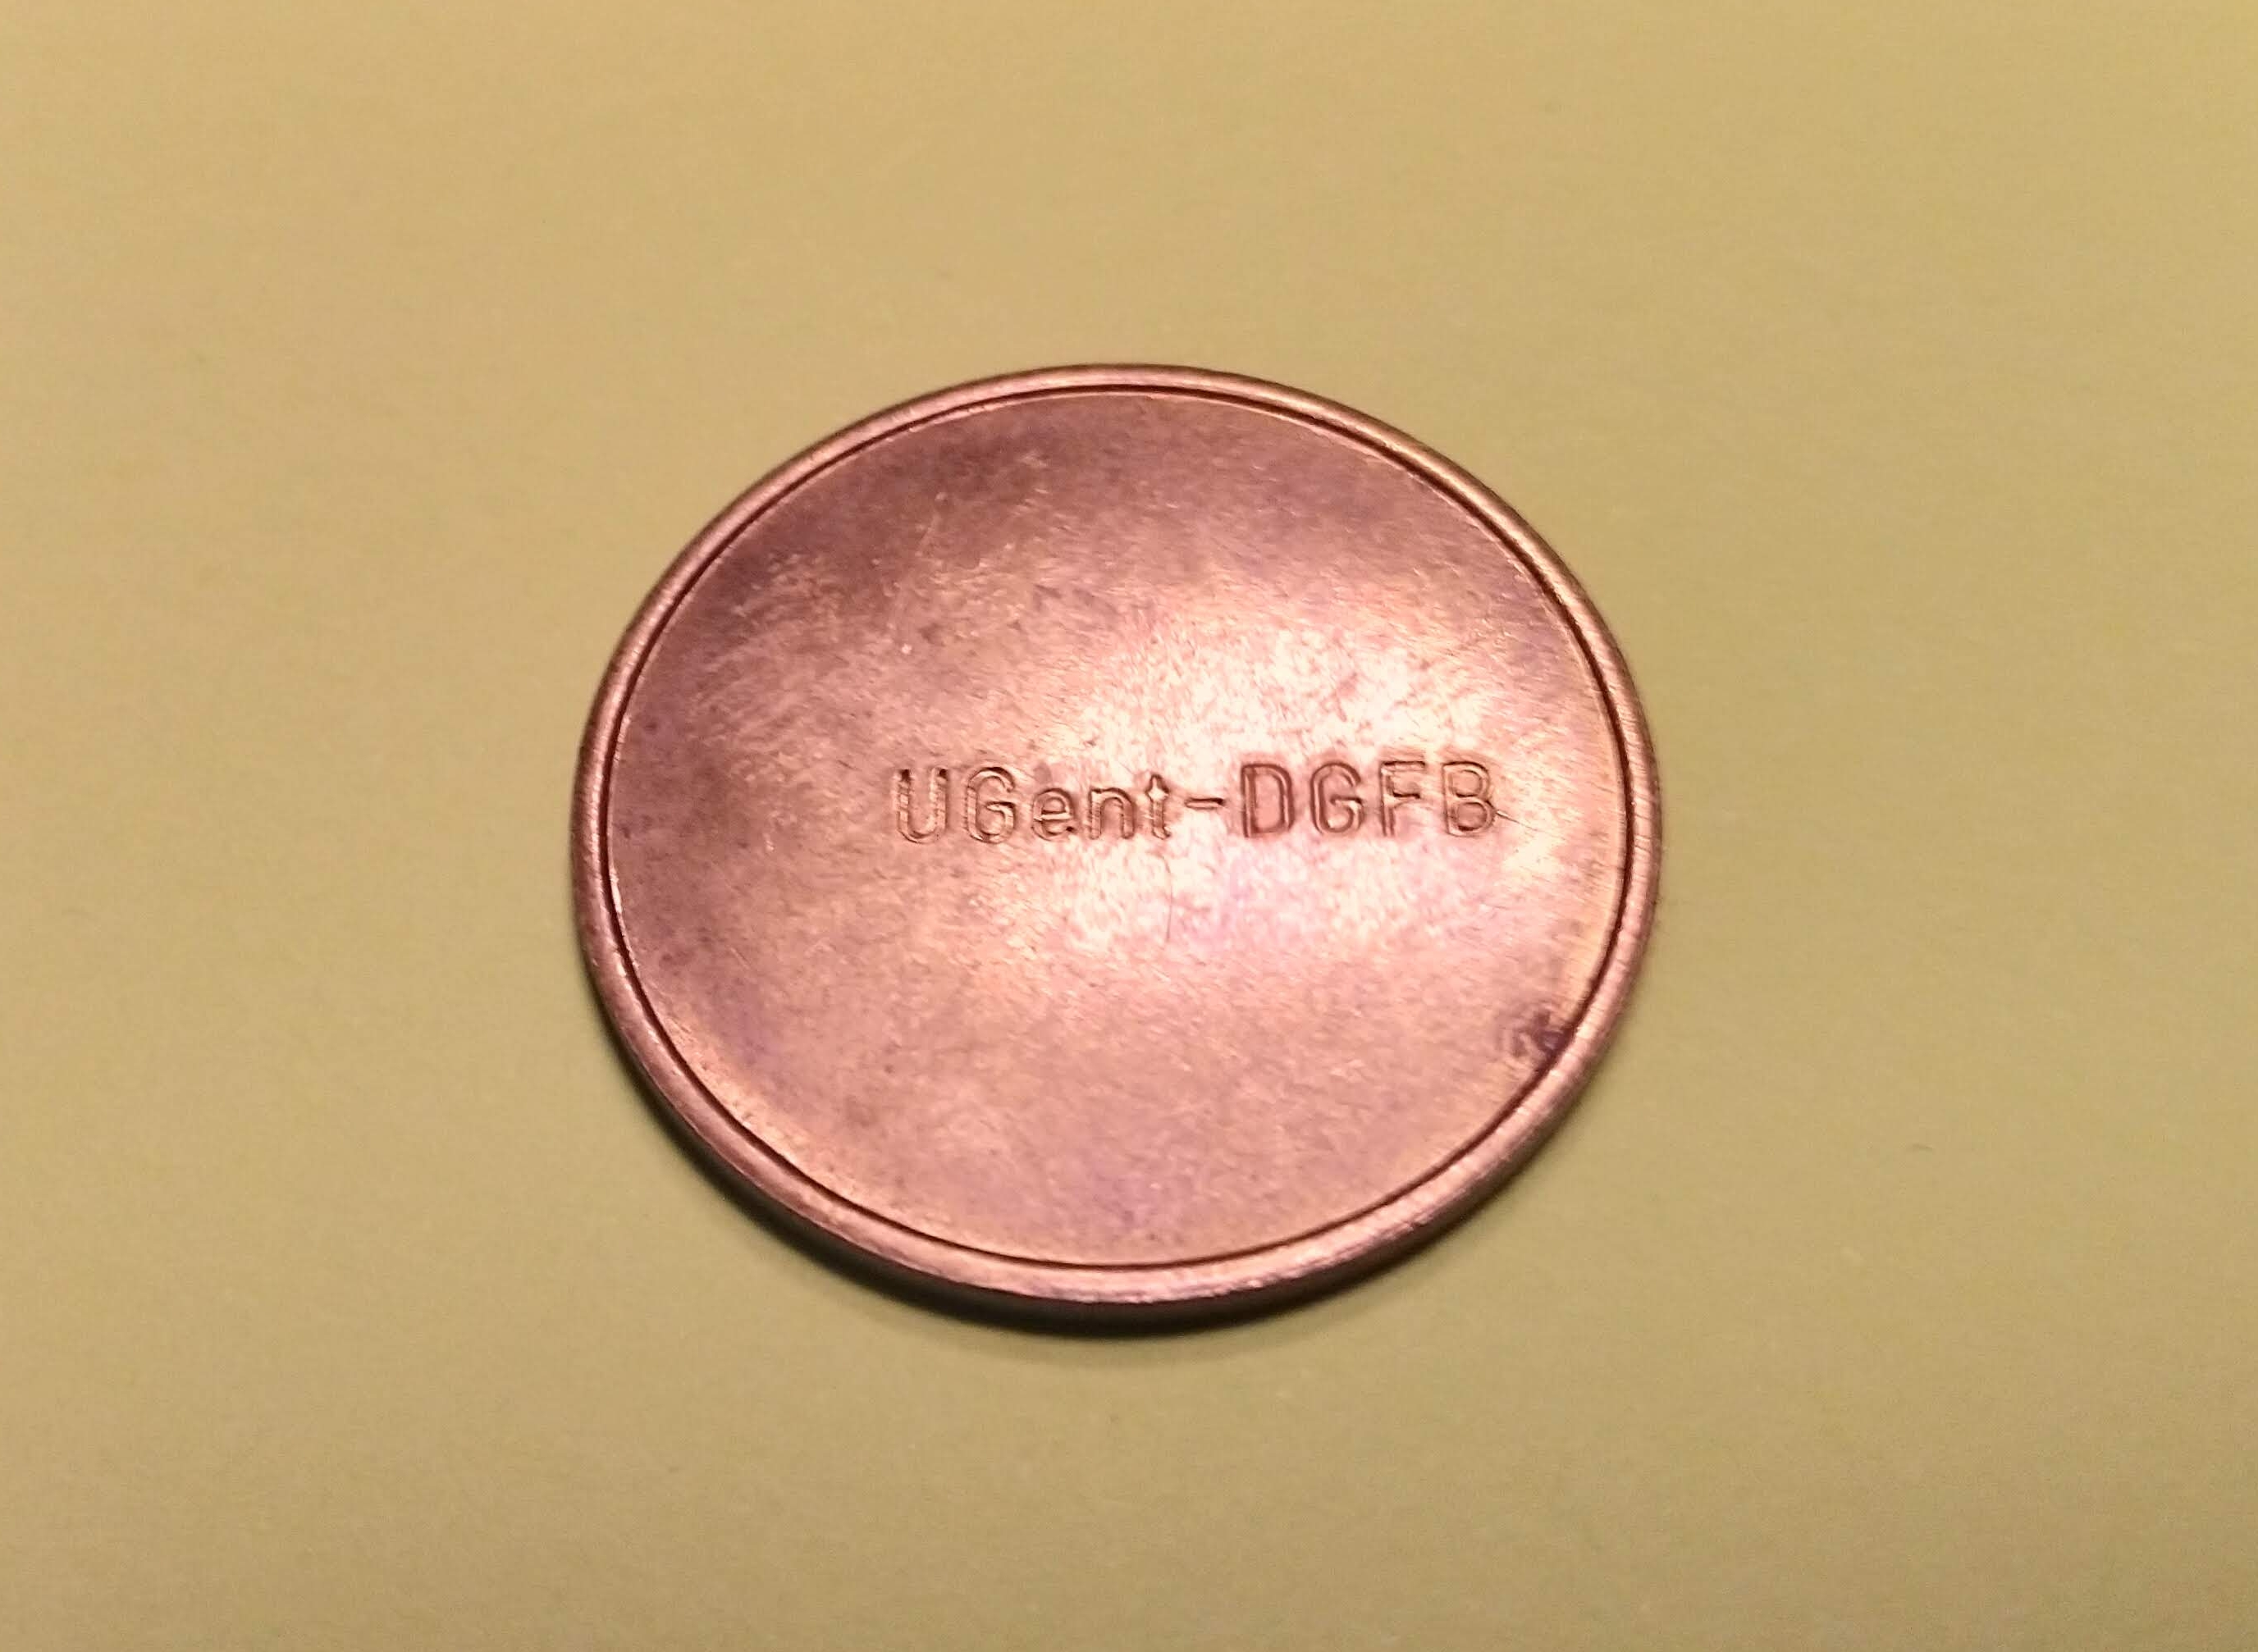
\includegraphics[width=0.5\linewidth]{img/token.jpg}
	\caption{Een huidige toegangstoken voor de parking van UGent te kunnen verlaten.}
\end{figure}

\subsubsection{Radio frequency Identification}

%Wat is RFID
Radio frequency Identication (RFID) is een technologie die aan de hand van elektromagnetische golven objecten kan identificeren. Dit met het voordeel dat er geen direct contact of zicht moet zijn tussen de scanner en het object. RFID gebeurt a.d.h.v een RFID reader en een RFID tag. De reader zendt een elektromagnetisch signaal uit. De tag ontvangt deze golven en kan op zijn beurt de opgevraagde informatie verzenden. \autocite{li2009design}

%RFID op UGent
Aan iedere uitgang op UGent zijn RFID-kaartlezers te vinden. Deze zijn voorzien om een vlotte toegang te verlenen aan werknemers en worden via een centraal beheerd systeem.

Het is geen optie om rfid voor alle bezoekers te gebruiken aangezien er vaak bezoekers binnentreden die maar 1 dag op de campus zijn. In dat geval zou er voor iedere dagbezoeker een RFID-kaart moet gemaakt worden. Aangezien de prijs van een RFID-kaart over de 10 euro is, is het zeker geen optie om dit als oplossing te gebruiken.

\subsubsection{Barcodes}
In een poging tot de tokens te vervangen heeft UGent één uitgang op de parking UFO en het rectoraat waar barcodes worden gebruikt. Deze worden eerst geprint op de campus zelf, waarna de gebruiker de barcode in een slikker kan invoeren en toegang krijgen om de parking te verlaten.

Deze barcodes hebben het grote voordeel dat ze goedkoper zijn in het gebruik. Maar hebben ze nog steeds het probleem dat iedere gebruiker telkens aan het onthaal een nieuw ticket moeten opvragen, en dat er slikkers slikkers aanwezig moeten zijn die tijdelijk geleegd worden.

Volgende lijst dient als een verduidelijking van de nadelen:
\begin{itemize}
	\item Milieubelasting, verspilling van papier
	\item ofwel moet een papierslikker geledigd worden ofwel zal er vervuiling zijn van achtergelaten papier aan de uitgang.
	\item Op diverse plaatsen moeten er drukkers aanwezig zijn.
\end{itemize}


\subsection{Mogelijkheid van ANPR}
De vorige technologieën zijn weliswaar niet de enige mogelijke oplossing tot dit probleem.

Automatic Number Plate Recognition (ANPR) is de techniek om automatisch nummerplaten te herkennen. Deze techniek wordt al sinds 1976 gebruikt voor voor de detectie van gestolen wagens \autocite{uk2011anpr}. Hedendaags is ANPR al veel toegankelijker en kan het op vele plaatsen teruggevonden worden zoals bij bv. trajectcontrole \autocite{de2014snelheidscamera}, parkeersystemen, etc.
\par
ANPR heeft nog vele andere acroniemen zoals Automatic License Plate Recognition (ALPR), Automatic Vehicle Identification (AVI), Vehicle Plate recognition (VLPR), Vehicle Recognition Identifier (VRI), Car plate Recognition (CPR) en Car Plate Reader (CPR) \autocite{axis2019license}. In dit onderzoek zal voor nummerplaatdetectie het acroniem ANPR gebruikt worden.
\par
%Voordelen
Het gebruik van ANPR brengt enkele voordelen met zich mee:
\begin{itemize}
	\item Het is heel modulair; mensen kunnen een dagpas of toegang voor een volledig schooljaar krijgen.
	\item Er moet slechts éénmalig aangemeld worden om toegang voor een langere periode te krijgen. Dit zou helemaal digitaal gedaan kunnen worden, wat personeelskosten bespaart.
	\item Indien succesvol geïmplementeerd kan ANPR opstoppingen aan toegangspunten verminderen omdat er geen menselijke interactie met het systeem meer nodig is.
\end{itemize}
\par
%Nadelen
ANPR zelf komt ook met enkele nadelen.
\begin{itemize}
	\item Er is een centraal systeem nodig om de toegang van de nummerplaten te beheren.
	\item Ieder toegangspunt moet een internetvoorziening hebben om met het centrale systeem te communiceren.
	\item Iedere ANPR-camera moet correct ingesteld zijn om haalbare resultaten te behalen.
	\item Weersomstandigheden bieden extra moeilijkheid voor de detectie van nummerplaten (dag, nacht)
	\item Hedendaagse ANPR-camera's zijn een redelijke investering.
\end{itemize}
\par
Voor de herkenning van nummerplaten zijn een aantal technologieën beschikbaar. Deze werken adhv. Artificial Intelligence (AI) en zijn specifiek getraind op het detecteren en uitlezen van nummerplaten.
De technologie die in dit onderwerp gebruikt zal worden is OpenALPR, een Open-Source library gemaakt voor nummerplaatdetectie. Hiervoor is gekozen omdat OpenALPR een gratis Open-Source product is \autocite{openalprgithub}.
%Nadelen


\section{Privacy en GDPR}
\label{sec:privacy-en-gdpr}

Sinds 25 Mei 2018 is de General Data Protection Regulation (GDPR) in gang gezet, een regulatie die ingevoerd is om het huidige  en toekomstige digitale tijdperk veiliger te maken voor alle EU inwoners.
Deze wetgeving is gedreven op het concept dat privacy een mensenrecht is, en dat online-data ook zo behandeld moet worden. Dit is data die direct of indirect gelinkt kan worden aan een individu zoals locatie-data, cookies en ip-adressen \autocite{goddard2017eu}.

Hierdoor komen er een groot aantal extra regels op bedrijven te liggen, zo zijn ze bvb. verplicht om te toestemming vragen om persoonsgegevens te mogen verwerken. Dit is merkbaar online, waar vele sites toestemming vragen om advertentie-cookies te mogen opslaan. Een heleboel andere regels zijn er ook bijgekomen, wat het moeilijk kan maken om een nieuw systeem te maken die aan al deze voldoet.

\section{Hardware}
Om deze nummerplaatdetectie uit te voeren is gekozen voor een Raspberry PI Model B+. Deze hardware wordt vandaag de dag veel gebruikt bij IOT-applicaties door zijn lage kost en gemakkelijke bruikbaarheid.  

De Raspberry PI Model B+ beschikt over een 1.4GHz quad-core processor, 1GB LPDDR2 RAM, een on-board WiFi-kaart en de mogelijkheid om een Raspberry Pi Camera te verbinden \autocite{raspberrypisitemodelbplus} .

\subsection{Camera}
De camera die gebruikt wordt is een Pi-NoIR camera. Deze camera is ook geproduceerd door de Raspberry Pi Foundation en biedt afbeeldingen en video in een 8-MegaPixel formaat. In dit onderzoek is voor deze camera gekozen omdat deze makkelijk te verbinden is met de Raspberry Pi, relatief goedkoop is en geen IR-filter heeft. Dit maakt de camera direct ook interessant voor foto's te nemen in donkere omgevingen. \autocite{raspberrypisitemodelpinoir}

\section{Software}
De software die gebruikt wordt in dit onderzoek is het open-source framework OpenALPR. Deze software is geschreven om nummerplaatdetectie uit te voeren en kan video's en foto's verwerken in een groot aanbod van programmeertalen \autocite{openalprgithub}. De keuze voor deze software is gemaakt door Vado-Solutions omdat OpenALPR open-source is, wat kosten dekt. Verder kan deze software ook gebruikt worden op Linux, wat noodzakelijk is om dit onderzoek uit te voeren met een Raspberry Pi.
%%=============================================================================
%% Methodologie
%%=============================================================================

\chapter{Methodologie}
\label{ch:methodologie}

%% TODO: Hoe ben je te werk gegaan? Verdeel je onderzoek in grote fasen, en
%% licht in elke fase toe welke stappen je gevolgd hebt. Verantwoord waarom je
%% op deze manier te werk gegaan bent. Je moet kunnen aantonen dat je de best
%% mogelijke manier toegepast hebt om een antwoord te vinden op de
%% onderzoeksvraag.

\lipsum[21-25]



% Voeg hier je eigen hoofdstukken toe die de ``corpus'' van je bachelorproef
% vormen. De structuur en titels hangen af van je eigen onderzoek. Je kan bv.
% elke fase in je onderzoek in een apart hoofdstuk bespreken.


\chapter{\IfLanguageName{dutch}{Wetgeving omtrent nummerplaatdetectie}{Technical details about ANPR in the GDPR}}
\label{ch:wetgeving-nummerplaatdetectie}

Het is vanzelfsprekend dat er enkele wetgevingen zijn die slaan op nummerplaatdetectie, het nemen van foto's als toegangssysteem is een pak meer privacyingrijpend dan een token in te werpen. Sinds de nieuwe wet van de GDPR moet hier dan ook veel voorzichtiger mee omgesprongen worden.

In de volgende onderdelen wordt er beschreven wat deze wet inhoudt en op welke manier nummerplaatdetectie hieronder valt.

\section{Algemene verordening gegevensbescherming}
%Wanneer is gdpr van toepassing
De General Data Protection Regulation (GDPR) of in het Nederlands: Algemene Verordening Gegevensbescherming (AVG), is een nieuwe wetgeving die op 25 mei 2018 ingevoerd is met als doel regels op te stellen om de grondrechten en de fundamentele vrijheden van natuurlijke personen te beschermen in de Europese Unie, dit met name op hun recht op bescherming van persoonsgegevens. \autocite{avg2018privacy}

Voor de verwerking van deze gegevens worden maatregelen opgelegd over hoe deze op een correcte manier behandeld moeten worden en aan welke eisen een bedrijf moet voldoen indien deze hiermee handelt.

In dit onderdeel zal niet de volledige GDPR beschreven worden, maar enkel de onderdelen m.b.t. een parkeersysteem met nummerplaatdetectie.

\subsection{Definities}

\paragraph{Persoonsgegevens}
In artikel 4 van het GDPR worden persoonsgegevens als volgt beschreven: 'alle informatie over een geïdentificeerde of identificeerbare natuurlijke persoon ("de betrokkene"); als identificeerbaar wordt beschouwd een natuurlijke persoon die direct of indirect kan worden geïdentificeerd, met name aan de hand van een identificator zoals een naam, een identificatienummer, locatiegegevens, een online identificator of van een of meer elementen die kenmerkend zijn voor de fysieke, fysiologische, genetische, psychische, economische, culturele of sociale identiteit van die natuurlijke persoon' \autocite{avg2018privacy}

Hieruit blijkt dat nummerplaten onder de term persoonsgegevens vallen; Deze zijn geregistreerd aan een persoon en kunnen worden gebruikt om de persoon te identificeren. In een parkeersysteem met nummerplaatdetectie zal hier dus ook op gelet moeten worden. 

Artikel 5 van GDPR, 'persoonsgegevens moeten worden verwerkt op een wijze die ten aanzien van de betrokkene rechtmatig, behoorlijk en transparant is ("rechtmatigheid, behoorlijkheid en transparantie")` \autocite{avg2018privacy}.

\paragraph{Betrokkene}
De betrokkene is een geïdentificeerde of identificeerbare natuurlijke persoon die de vermelde persoonsgegevens bezit.

\paragraph{Verwerking van gegevens}
Een verwerking is een veel vermelde term in de GDPR en omvat een duidelijke definitie. Het verwerken van gegevens omvat eender welke operaties die op persoonsgegevens worden uitgevoerd. Waarvan het verzamelen, vastleggen, organiseren, raadplegen of vernietigen van deze gegevens onderdeel is. Deze lijst wordt verder uitgebreid omschreven in Artikel 4 punt 2 van de GDPR.

Indien een ANPR-systeem foto's neemt van auto's dan voert deze enkele verwerkingen uit. Deze zijn het vastleggen, raadplegen en mogelijks vernietigen van de gegevens. Ookal duurt dit proces maar enkele seconden en wordt er niets opgeslaan is er wel degelijk sprake van een verwerking.

\paragraph{Verwerkingsverantwoordelijke}
De verwerkingsverantwoordelijke is een persoon die instaat voor het correct verwerken van gegevens. Hij bepaalt het doel en de middelen van de verwerking. Op vraag van overheidsinstanties moet hij kunnen aantonen waarom en hoe de verwerking wordt uitgevoerd.

\paragraph{Verwerker}
Een verwerker is een persoon die persoonsgegevens verwerkt in opdracht van de verwerkingsverantwoordelijke.

\subsection{Beginselen inzake gegevensverwerking}
Het is niet mogelijk om zomaar om het even welke persoonsgegevens te verwerken. De GDPR stelt enkele regels op die organisaties moeten naleven voor het verwerken van gegevens. De verwerkingsverantwoordelijke moet kunnen aantonen dat deze nageleefd worden. De beginselen inzake gegevensverwerking zijn te vinden in Artikel 5 van de GDPR.

\paragraph{Rechtmatigheid van verwerking}
\label{rechtmatigheid-van-verwerking}
Een verwerking van persoonsgegevens dient ten alle tijden rechtmatig te zijn, indien dit niet het geval is kunnen er sancties optreden.

In artikel 6 beschrijft de GDPR enkele voorwaarden waar minstens aan voldaan moet worden. Zo kan de betrokkene toestemming gegeven hebben, is er een wettelijke plicht of zijn er gerechtvaardigde belangen voor de verwerking van de gegevens.

In het geval van een ANPR-camera is het niet mogelijk om toestemming aan de betrokkene te vragen. Dit omdat toevallige voorbijgangers ook de camera kunnen triggeren welke vervolgens hun gegevens verwerkt, waarvoor deze geen toestemming hebben kunnen geven. Hiervoor is de enige echte optie het gerechtvaardigd belang.

Het gerechtvaardigd belang berust erop dat de belangen van de verwerking meer doorwegen dan de belangen van de betrokkene. En dat dit belang enkel kan behartigd worden door persoonsgegevens te verwerken \autocite{autoriteit2019gerechtvaardigd}.

\paragraph{Doelbinding}
De doeleinden voor de gegevensverwerking dienen uitdrukkelijk omschreven en gerechtvaardigd te zijn. Geen verdere verwerking is toegestaan die niet aan deze doeleinden beantwoordt.

\paragraph{Dataminimalisatie en juistheid}
De opgeslagen data dienen beperkt te zijn tot wat nodig is om de beschreven doeleinden te voldoen. Het is de bedoeling om een strikt minimum van data bij te houden. Verder moet de data actueel gehouden worden en indien onjuist, verwijderd of gerectificeerd te worden.

\paragraph{Opslagbeperking}
Indien de betrokkene identificeerbaar is, mag de data niet langer opgeslaan worden dan dat deze nodig is voor het verwezenlijken van de doeleinden.

\paragraph{Integriteit en vertrouwelijkheid}
De verwerking dient genoeg beveiligd te zijn door gebruik te maken van passende, technische en organisatorische maatregelen. Verder dient deze beschermd te zijn tegen iedere niet toegelate of onwettige verwerking, verlies, vernietiging of kwaliteitsverlies van de gegevens.

\paragraph{Verantwoordingsplicht}
De verwerkingsverantwoordelijke is verantwoordelijk voor de naleving van deze beginselen van de verordening. Hij moet dan ook ten alle tijde kunnen aantonen dat aan deze beginselen voldaan zijn.


\subsection{Rechten van de betrokkene}
\label{rechten-betrokkene}
Vervolgens stelt de GDPR enkele uitgebreide rechten op die de betrokkene, de eigenaar van de persoonsgegevens, heeft. Deze zijn terug te vinden in hoofdstuk 3 van de GDPR en zijn omschreven in de volgende punten.

\paragraph{Recht om geïnformeerd te zijn}
Indien een ANPR-systeem is opgesteld, dient er volgens artikel 13 van de GDPR, gesignaleerd te worden dat een dergelijk systeem aanwezig is, dit tezamen met contactinformatie van de verwerkingsverantwoordelijke, de verwerkingsdoeleinden waarvoor de persoonsgegevens zijn bestemd en de rechtsgrond van de verwerking \autocite{besafe2018picto}. Het verplichte pictogram voor camerasignalisatie is te zien in Figuur \ref{anpr-aanduiding}.

Deze signalisatie moet vanaf een duidelijke afstand zichtbaar zijn zodat de betrokkene deze kan lezen vooraleer hij de gemonitorde omgeving betreedt. Deze omgeving moet duidelijk zijn voor de betrokkene zodat hij deze kan mijden.

\begin{figure}[h!]
	\centering
	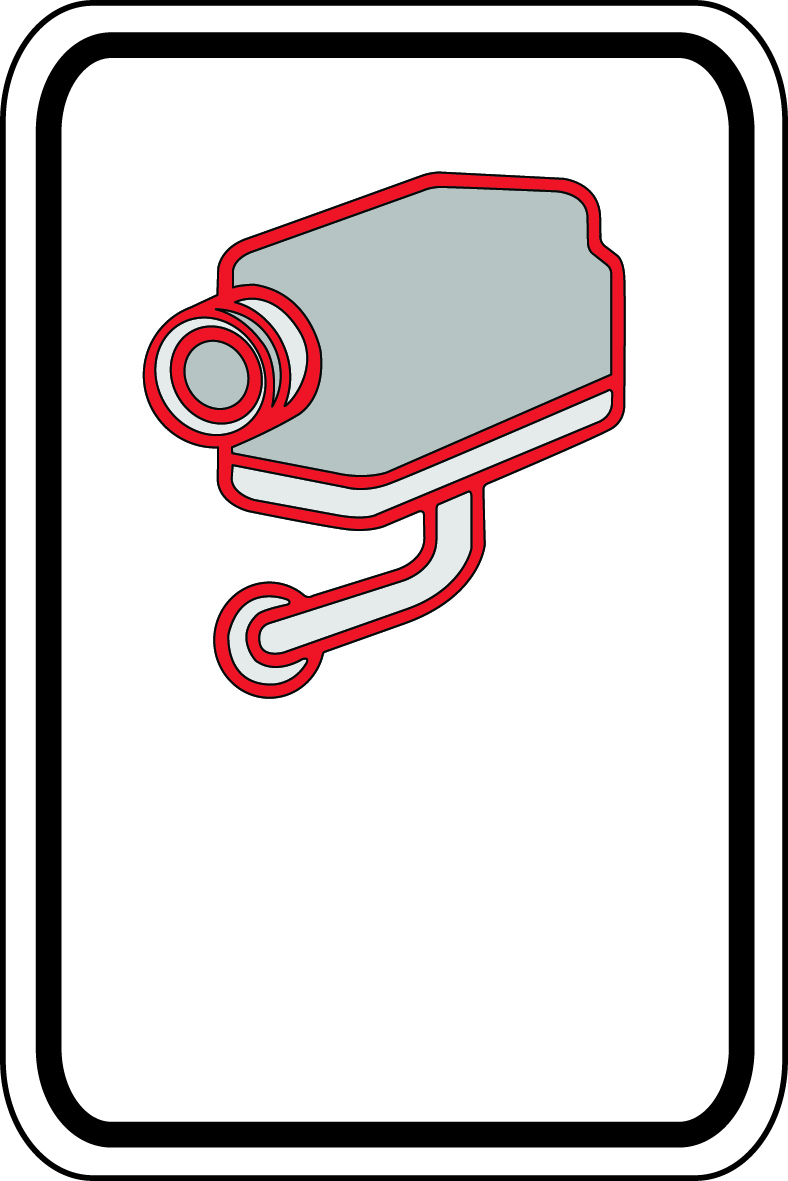
\includegraphics[width=.5\linewidth]{img/anpr-aanduiding.png}
	\caption{Belgisch pictogram voor camera-aanduiding. \autocite{besafe2018picto}}
	\label{anpr-aanduiding}
\end{figure}

\paragraph{Recht op informatie en rectificatie van persoonsgegevens} 
Iedereen bezit zijn eigen persoonlijke data en mag deze bijgevolg ook inkijken en corrigeren. Indien een gebruiker vraagt om zijn persoonsgegevens in te kijken, moet het bedrijf in kwestie al de persoonsgegevens van de gebruiker binnen de maand kunnen opleveren. Ook kan een gebruiker eender wanneer beslissen om al zijn data te laten verwijderen \autocite{avg2018privacy}. Dit is terug te vinden in artikel 15 en 16 van de GDPR.

\paragraph{Recht op vergetelheid}
Een verwerkingsverantwoordelijke is verplicht persoonsgegevens zonder onredelijke vertraging te wissen indien deze niet meer nodig zijn voor de oorspronkelijke doeleinden, de gegevens onrechtmatig verwerkt zijn of de betrokkene zijn toestemming intrekt. Enkel indien één van de uitzonderingen in artikel 17 (3) van toepassing zijn kan dit langer duren. \autocite{edpb2019guidelines}

\paragraph{Recht op beperking van verwerking}
Bij camerasystemen die berusten op het gerechtvaardigd belang of openbaar belang om data te verwerken, heeft een betrokkene het recht om op eender welk moment hier bezwaar tegen te maken. Indien de verwerkingsverantwoordelijke geen legale gronden kan voorleggen die zwaarder doorwegen dan de rechten van de betrokkene, is hij verplicht aan de wensen van de betrokkene te voldoen. Dit is terug te vinden in artikel 18 van de GDPR.

In een context van camerabewaking kan deze objectie gemaakt worden voor, tijdens, of na een betrokkene een bewaakte zone betreedt. Dit betekent dat indien de belangen van de verwerkingsverantwoordelijke niet doorwegen op de rechten van de betrokkene, de camera direct moet kunnen stopgezet worden zodanig dat er geen beelden van de betrokkene meer worden gemaakt. Anderzijds is het ook mogelijk om de gemonitorde zone genoeg af te bakenen zodat de verwerkingsverantwoordelijke de toestemming kan verifieren alvorens de betrokkene deze betreedt. \autocite{edpb2019guidelines}

%\subsection{Data Protection Officer}
%Een Data Protection Officer (DPO) moet aangesteld worden, Nederlands: Functionaris voor gegevensbescherming. NIET NODIG VOOR KLEINE ORGANISATIE

\subsection{Verwerking waarvoor identificatie niet vereist is}
Artikel 11 van de GDPR zegt dat indien de doeleinden niet vereisen dat de betrokkene geïdentificeerd is, dat de verwerker geen aanvullende gegevens hoeft bij te houden.
\par
Hieruit volgt dan ook dat indien de verwerker kan aantonen dat hij de betrokkene niet kan identificeren, artikelen 15 tot en met 20, beschreven in onderdeel \ref{rechten-betrokkene} niet meer van toepassing zijn.

\subsection{Functionaris voor gegevensbescherming}
Een functionaris voor gegevensbescherming of data protection officer (DPO) is iemand met deskundingheid op het gebied van gegevensbescherming. Een DPO wordt aangewezen om de verwerkingsverantwoordelijke of de verwerker te informeren en adviseren over hun verplichtingen van de GDPR en andere wetten over gegevensbescherming.

\paragraph{Voorwaarden voor het aanstellen}
Een DPO dient aangesteld te worden in volgende gevallen:
\begin{itemize}
	\item De verwerking wordt verricht door een overheidsinstantie of overheidsorgaan.
	\item De verwerker is hoofdzakelijk belast met verwerkingen die observatie op grote schaal van betrokkenen eisen.
	\item De verwerker is hoofdzakelijk belast met het verwerken van uitzonderlijke persoonsgegevens.
\end{itemize}

Er kan verondersteld worden dat het verwerken van persoonsgegevens over twee campussen niet groot genoeg is om een DPO aan te stellen.

\paragraph{Taken}
De DPO dient de verwerkingsverantwoordelijke of de verwerker te informeren en adviseren over hun rechten en verplichtingen, het toezien op het naleven van de GDPR, samenwerken met de toezichthoudende autoriteit en optreden als contactpunt voor de toezichthoudende autoriteit.


\section{Belgische Camerawetgeving}
Sinds 25 mei 2018 is de nieuwe camerawetgeving ingevoerd, dit is een herziening van de Camerawetgeving uit 2007 en viel niet toevallig samen met de dag dat de GDPR is ingevoerd. Deze wet slaat op bewakingscamera's en geldt enkel wanneer deze als doel hebben:
\begin{itemize}
	\item Misdrijven tegen personen of goederen te voorkomen, vast te stellen of op te sporen;
	\item overlast in de zin van artikel 135 van de nieuwe gemeentewet, te voorkomen, vast te stellen of op te sporen, de naleving van gemeentelijke reglementen te controleren of de openbare orde te handhaven.
\end{itemize}
Aangezien nummerplaatdetectie als toegangssysteem geen van deze doelen bevat valt het niet onder de camerawetgeving voor bewakingscamera's. \autocite{staatsblad2007wet}

Natuurlijk zal er wel nog rekening gehouden moeten worden met de GDPR omdat er persoonsgegevens worden verwerkt door een bedrijf, vereniging of eenmanszaak. \autocite{gba2019videoparlofoon}

\section{Openbare weg}
Indien de camera een deel van de openbare weg waarneemt, dan moet er een aanvraag ingedient worden bij de politie, waarna dit wordt vastgelegd in de gemeenteraad. \autocite{beltug2018camerawet}

Aangezien het een hele administratie is om dit in orde te brengen, kan het bedrijf het beeld van de openbare weg van de camera 'blacken'. Dit moet niet enkel op het beeld van de camera gebeuren, maar ook op de opgeslagen data. \autocite{beltug2018camerawet}

\section{Toegepast op een ANPR-systeem}
De GDPR is een uitgebreide wetgeving die vele voorwaarden opstelt voor het verwerken van persoonsgegevens. Het is niet mogelijk om een volledige checklist te geven, maar enkele basisrichtlijnen geven een goed beeld van de mogelijkheid om dit te implementeren. Een ANPR-systeem brengt een pak meer persoonsgegevens met zich mee dan een simpel tokensysteem of RFID-systeem.

Indien men een ANPR-systeem wilt implementeren, zullen alle reguleringen rond de verwerkte gegevens moeten voldaan worden. Dit wordt in de volgende punten verduidelijkt.

\subsection{Een verwerking dient gerechtigd te zijn.}
Ieder contact met gegevens, of het nu lezen, verwijderen of verplaatsen is, is een verwerking. Indien men geen gewettigde reden heeft om de data te verwerken, riskeert u om hierop beboet te worden. Ga dus na op welke basis u data wilt verwerken en zorg dat u deze rechtmatigheid kan bevestigen.

Er zijn enkele gronden waardoor het gerechtigd is om persoonsgegevens te verwerken. In onderdeel \ref{rechtmatigheid-van-verwerking} is reeds beschreven hoe een dergelijk camerasysteem het best rust op de het gerechtvaardigde belang, waarbij de belangen van de verwerking meer doorwegen dan de belangen van de betrokkene. 

\subsection{Verwerk enkel de data die benodigd is voor uw doeleinden.}
Dataminimalisatie berust erop dat u geen data verwerkt dat u niet nodig hebt om uw doelen te bereiken. Indien u bijvoorbeeld een ANPR-systeem opstelt als toegangssysteem, dient u geen foto's van toevallige voorbijgangers bij te houden.

\subsection{Informeer dat persoonsgegevens verwerkt worden.}
Het bekende artikel 13 berust erop dat een betrokkene kennis heeft dat zijn gegevens verwerkt worden. Informeer dus duidelijk dat cameradetectie aanwezig is en vermeld een contactpersoon voor vragen.

\subsection{Wees bereid om gegevens op te vragen en aan te passen op vraag van derden.}
Niet enkel de betrokkene, maar ook de overheid heeft het recht om eender wanneer zijn toebestemde persoonsgegevens op te vragen of aan te passen. Deze moeten binnen een tijdspanne van een maand volbracht worden om boetes te vermijden.

Indien mogelijk kunnen de bekomen gegevens geanomiseerd worden zodat geen betrokkenen kunnen worden geïdentificeerd. Indien de betrokkenen niet kunnen geïdentificeerd worden, kan u deze data ook niet opleveren op aanvraag.

\subsection{Stel een contactpersoon aan.}
Iemand binnen de organisatie moet aangesteld zijn om na te gaan of persoonsgegevens op een correcte manier verwerkt worden. Deze is verantwoordelijk indien de GDPR of andere privacy reguleringen niet nageleefd worden.

Indien mogelijk kan een Data-Protection Officer aangesteld worden. Deze is een vereiste bij grootschalige projecten waarbij zijn taak hoofdzakelijk het valideren is dat de GDPR nageleefd wordt. Deze dient gemakkelijk te contacteren te zijn vanuit eender welke vestiging.

\subsection{Is het mogelijk om aan deze eisen te voldoen?}
De co-promotor van dit onderzoek, Vado-Solutions, heeft reeds een idee van een implementatie. Hun systeem zou toegang verlenen voor een nummerplaat voor een bepaalde duur, bv. een bezoeker die een maand lang toegang tot de campus zou moeten hebben. Door enkel de nummerplaat en de periode op te slaan wordt er een groot deel van het extra papierwerk rond de GDPR omzeild.

Verder zouden de genomen foto's niet worden opgeslaan in het systeem. De analyse van de foto's gebeurt onmiddelijk, waarna ze verwijderd worden. Dit geeft het voordeel dat hier geen databank van moet worden bijgehouden en dat er geen extra werk in kruipt op vlak van GDPR. Indien een betrokkene zijn foto's zou willen laten verwijderen is het onmogelijk, er worden namelijk geen foto's opgeslagen.

Enkel op vlak van het nemen van foto's zou er nog moeten beschreven worden hoe dit exact valt onder het gerechtvaardigd belang. Dit is namelijk de enigste grond waarop een dergelijk ANPR-systeem gerechtigd zou kunnen zijn.

Als besluit zou deze zeer minieme oplossing zeker mogelijk zijn om te implementeren op de campussen. De kleine voetafdruk van persoonlijke gegevens verminderen de lasten van de GDPR en zolang de schaal over enkele campussen blijft zou er geen DPO moeten worden aangesteld worden, wat kosten bespaart. Indien men een checklist wenst uit te voeren biedt gdpr.eu een degelijke checklist aan op https://gdpr.eu/checklist/.

%\subsection{Aangifte van camera's}
%Iedere bewakingscamera moet via het E-loket op http://www.aangiftecamera.be aangegeven worden. \autocite{besafe2018bewakingscameras}

%\subsection{Register}
%Sinds de GDPR die de privacywetgeving vervangt hoort er geen aangifte bij de Gegevensbeschermingsautoriteit plaats te vinden, maar wel de de verantwoordelijke voor de verwerking een een register bijhoudt  voor de verwerkingsactiviteiten die onder haar verantwoordelijkheid vallen. Dit register moet op verzoek in beschikking gesteld worden van de Gegevensbeschermingsautoriteit. \autocite{besafe2018beeldverwerking}

%In dit register wordt bijgehouden wat de doeleinden zijn 


%\subsection{Bewaren van beelden}
%Bewaren van beelden mag maximaal 1 maand. 3 maanden in bedrijven met een verhoogd risico zoals luchthavens en havens.

\chapter{\IfLanguageName{dutch}{Maatregelingen voor nummerplaatdetectie met Raspberry PI}{Implementation guide for ANPR with Raspberry PI}}
\label{ch:maatregelingenraspberrypi}

In deze sectie beoordelen we welke maatregelingen genomen moeten worden bij het implementeren van een ANPR systeem met oog op de parking aan de UGent.

Nummerplaatdetectie is al sterk geevolueerd sinds vroeger, maar heeft nog steeds enkele drawbacks. Zo spelen factoren zoals weer, belichting en plaatsing van de camera's een invloed op de nauwkeurigheid van de uitlezingen.

zoals camerahoek, resolutie, weerstomstandigheden, belichting, afbeeldingcompressie, tijd voor een uitlezen. Door het volgen van deze maatregelingen kan een werknemer nummerplaatdetectie installeren op een zo'n correct mogelijke manier.

\section{Maatregelingen}

\subsection{Detectie}
Hoe weet men wanneer een nummerplaat te detecteren?
Ultrasone sensors, autodetectors ondergronds

\subsection{Camera Plaatsing}
infrarode camera nacht
Detectie snachts \autocite{boonsin2017car}
De belangrijkste factor op nauwkeurigheid van ALPR is plaatsing en kwaliteit van de camera \autocite{openalprcameraplacement}.

\paragraph{Locatie van de camera}
Uit een prototype van \textcite{arrieta2019prototype} bleek dat nummerplaten niet correct geidentificeerd werden bij een inclinatiehoek vanaf 30 graden. Het is dus aanbevolen om de camerahoek te beperken tot een kleine hoek.

Verder is het aangeraden om de camera hoger te plaatsen dan de koplampen van de auto, dit om te voorkomen dat de camera verblind wordt door het sterke licht.

OpenALPR heeft opties om de hoek te calibreren \autocite{openalprdocumentation}

\paragraph{Camera orientatie}
De camera hoort parallel met de randen van het scherm te staan. Dit omdat de algoritmes voor ANPR getraint zijn op detectie van horizontale nummerplaten, maar niet van gedraaide.

\paragraph{Pixeldichtheid}
Het aantal pixels van de foto waaruit een nummerplaat bestaat is van belang voor OpenALPR voor een duidelijke herkenning. Indien een foto van veraf is genomen zal deze laag zijn en van dichtbij zal deze dan weer hoog zijn. OpenALPR verwacht voor Europeaanse nummerplaten minstens een wijdte van 75 pixels en een grootte meer dan 250 pixels verhoogt niet opmerkelijk de accuraatheid. \autocite{openalprcameraplacement}

\subsection{Camera instellingen}
De belangrijkste factor van een performant ANPR-systeem is een correct ingestelde camera. Het nemen van foto's is de eerste stap in het proces en indien hierop geen nummerplaten duidelijk zijn kan OpenALPR onmogelijk iets detecteren. In dit onderdeel worden de belangrijkste instellingen verduidelijkt die bijdragen tot een correcte foto voor gebruik bij nummerplaatdetectie.

\paragraph{Shuttersnelheid}
\textcite{guo2017vehicle} stelt een trainingsmodel voor dat rekening houdt met blur.

camera shutterspeed is de snelheid dat een camera foto's neemt. In een klaarlichte dag kan de shutterspeed zo'n 1/10000 seconden halen terwijl in het donker dit wel een volle seconde kan duren om genoeg licht te behalen. \autocite{openalprcameraplacement}

Bij een lange shutterspeed kan het dus zijn dat een voertuig een meter vooruit is gereden, terwijl bij een kleine shutterspeed dit bv. maar een centimeter is. Een korte shutterspeed is dus interessant voor het implementeren van nummerplaatdetectie aangezien de auto minder ver is gereden en dus minder motion blur op de foto staat.

\begin{figure}[h!]
	\centering
	\begin{subfigure}[b]{0.4\linewidth}
		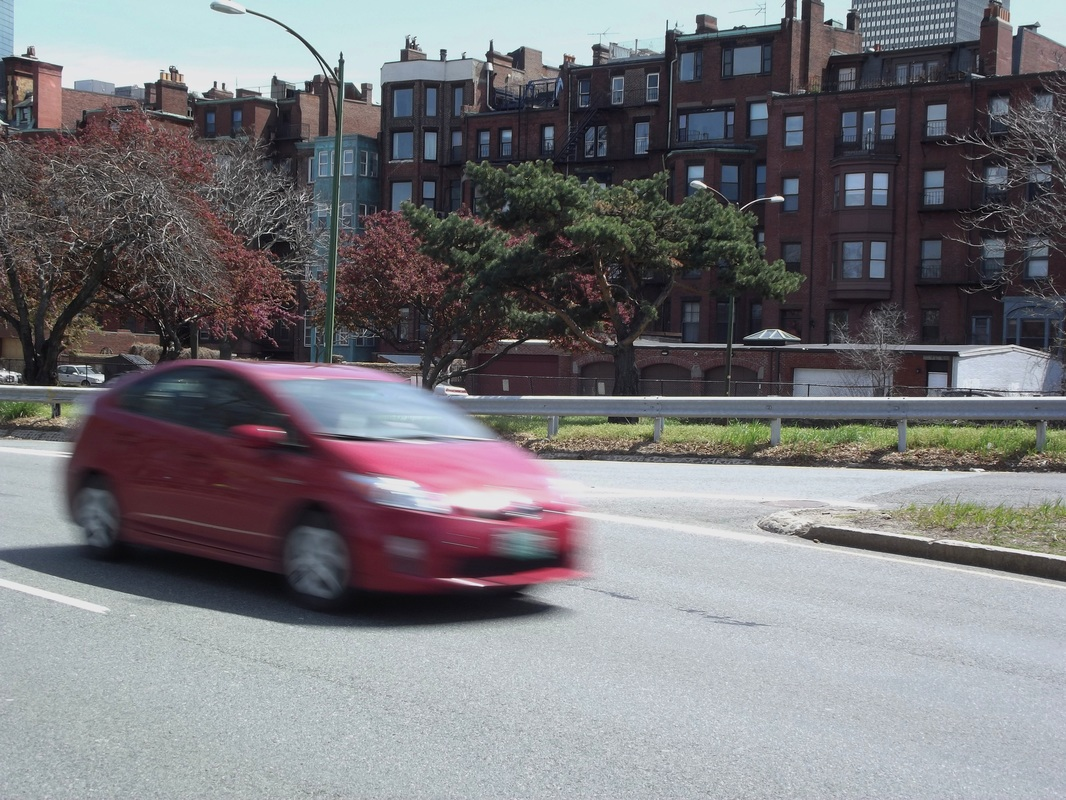
\includegraphics[width=\linewidth]{img/shutter-slow.jpg}
		\caption{Shutter speed van 1/60}
	\end{subfigure}
	\begin{subfigure}[b]{0.4\linewidth}
		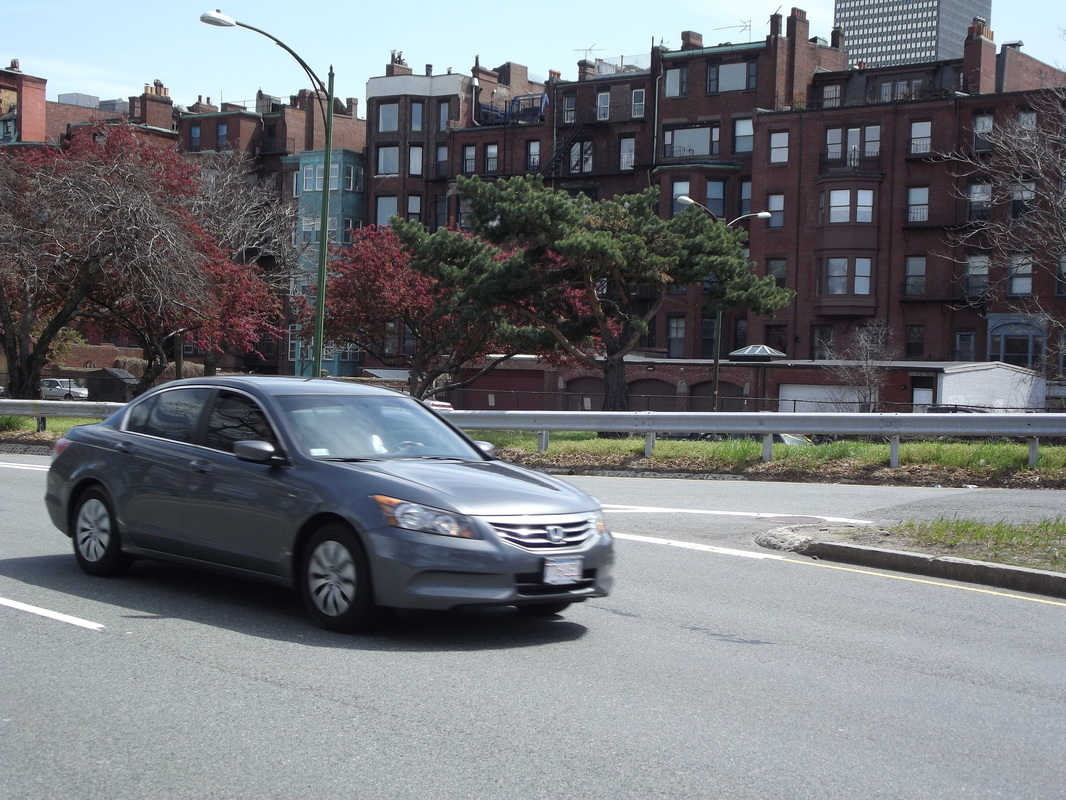
\includegraphics[width=\linewidth]{img/shutter-fast.jpg}
		\caption{Shutter speed van 1/250}
	\end{subfigure}
	\label{fig:ntlpc}
	\caption{Vergelijking van verschillende shutterinstellingen. \autocite{easy2019shutter}}
\end{figure}

Het nadeel van een kleine shutterspeed te nemen is dat er veel minder licht aanwezig is op de foto's, wat de detectie dan weer omlaag brengt. Zo krijg je 's nachts bijna volledig zwarte foto's. Dit kan geremedieerd worden door belichting bij te plaatsen.

\paragraph{Belichting}
'S nachts is de belichting van de nummerplaten een stoorzender, de camera kan onmogelijk een kleine shutterspeed aanhouden en een genoeg belichte afbeelding krijgen. Hiervoor moet er dus een eigen belichting bijgezet worden.

Zelfs al wordt er belichting bijgezet zal de nummerplaat spijtig genoeg niet leesbaar zijn, dit komt doordat de koplampen van een auto ervoor zorgen dat de camera niet eens een nummerplaat meer ziet. Een algemene oplossing voor deze problemen is het gebruik van een IR-camera. Een IR-camera detecteert enkel IR-licht en heeft dus geen invloed van de koplampen van wagens. Verder is het voordeel hiervan dat IR-licht niet zichtbaar is voor het menselijk oog, en dus ongestoort snachts en overdag gebruikt kan worden.

\begin{figure}[h!]
	\centering
	\begin{subfigure}[b]{0.4\linewidth}
		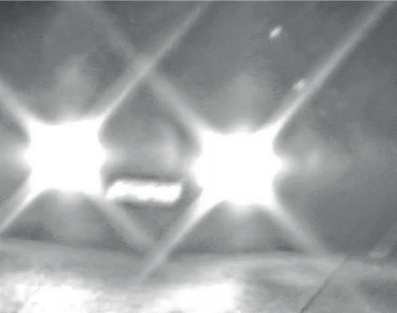
\includegraphics[width=\linewidth]{img/night-time-lpc-bad.png}
		\caption{Slecht geconfigureerde camera.}
	\end{subfigure}
	\begin{subfigure}[b]{0.4\linewidth}
		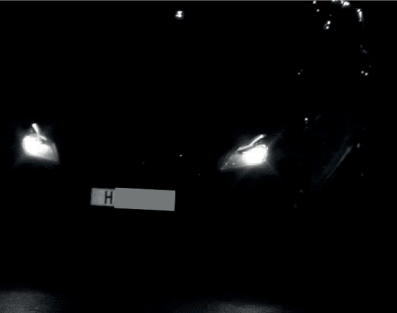
\includegraphics[width=\linewidth]{img/night-time-lpc-good.png}
		\caption{Correct geconfigureerde camera.}
	\end{subfigure}
	\label{fig:ntlpc}
	\caption{Vergelijking tussen camerainstellingen in de nacht. \autocite{axis2019license}}
\end{figure}
Infrarood, infraroodlamp, dag, nacht

\paragraph{Depth of field}
Focus van de camera.

\subsection{Legale maatregelingen}
\subsubsection{Buitenlandse nummerplaten}
OpenALPR heeft verscheidene configuraties voor Europa, Amerika en andere continenten. Bij een keuze van de Europese databank wordt er geen tot weinig fouten verwacht indien een nummerplaat van een ander land komt.

\subsubsection{Motoren}
Motoren hebben standaard geen nummerplaat aan hun voorkant. Dit kan opgelost worden door nummerplaatdetectie langs achteren te doen.
**Hebben motoren toestemming nodig om te parkeren?**

\subsection{OpenALPR}

\paragraph{Configuratie}
\textcite{arrieta2019prototype} en \textcite{buhus2016automatic} concluderen beiden dat openalpr standaard goede resultaten biedt, maar nog hogere resulaten bereikt kunnen worden indien er verduidelijkt wordt welk type nummerplaten er verwacht wordt. Dit houdt factoren in zoals de juiste dataset van het land gebruiken en de volgorde van de kentekenkarakters aanduiden.

Door pattern matching toe te passen kunnen resultaten nog nauwkeuriger zijn. Hierbij wordt een reguliere expressie op alle top N resultaten uitgevoerd en worden de non-matching resultaten verworpen.

\paragraph{Commerciele upgrades}
OpenALPR biedt commerciele versies van OpenALPR aan, deze zouden een hogere nauwkeurigheid bieden.

\section{Maatregelingen inzake UGent}
In dit deel gaan we na op welke wijze de maatregelingen toegepast kunnen worden op de campus van UGent.  
Motoren?
camera's aan ingangen?
waar camera plaatsen?

\subsection{Camera}
Als camera zal gebruik gemaakt worden van de PiNoIR-Cam. Deze camera is een standaard extensie voor de Raspberry-PI die geen infrarood filtering heeft staan. Standaard wordt infrarood uit afbeeldingen gefilterd omdat deze een ongewenst bijproduct zijn op foto's. De PiNoIR camera filtert geen infrarood uit de afbeeldingen en maken het dus mogelijk om te gebruiken voor infrarood detectie.

\paragraph{Cameraplaatsing}
Voor de plaatsing van de camera's wordt er gewenst zo veel mogelijk kosten te besparen en is de locatie van de hefboom een gewenste locatie. De camera zal zo hoog mogelijk aan de metalen constructie worden gehangen zodat deze zo min mogelijk interferentie heeft.

\paragraph{Cameraconfiguratie}
Shutterspeed

\chapter{\IfLanguageName{dutch}{Praktische uitvoering van nummerplaatdetectie op UGent}{Implementation of ANPR at UGent}}
\label{ch:praktischeUitvoering}

%%=============================================================================
%% Conclusie
%%=============================================================================

\chapter{Conclusie}
\label{ch:conclusie}

%% TODO: Trek een duidelijke conclusie, in de vorm van een antwoord op de
%% onderzoeksvra(a)g(en). Wat was jouw bijdrage aan het onderzoeksdomein en
%% hoe biedt dit meerwaarde aan het vakgebied/doelgroep? Reflecteer kritisch
%% over het resultaat. Had je deze uitkomst verwacht? Zijn er zaken die nog
%% niet duidelijk zijn? Heeft het onderzoek geleid tot nieuwe vragen die
%% uitnodigen tot verder onderzoek?

\lipsum[76-80]



%%=============================================================================
%% Bijlagen
%%=============================================================================

\appendix
\renewcommand{\chaptername}{Appendix}

%%---------- Onderzoeksvoorstel -----------------------------------------------

\chapter{Onderzoeksvoorstel}

Het onderwerp van deze bachelorproef is gebaseerd op een onderzoeksvoorstel dat vooraf werd beoordeeld door de promotor. Dat voorstel is opgenomen in deze bijlage.

% Verwijzing naar het bestand met de inhoud van het onderzoeksvoorstel
%---------- Inleiding ---------------------------------------------------------

\section{Introductie} % The \section*{} command stops section numbering
\label{sec:introductie}

Parkings zijn van groot belang in het dagelijks leven. Iedere dag rijden talloze wagens naar hun plaats om daar na een achttal uren weer opgepikt te worden. Ieder van deze wagens moet zich dan ook telkens identificeren om deze te betreden of te verlaten. Dit doen ze met behulp van tickets, badges of andere toegangssystemen. Ieder systeem heeft zijn eigen voor- en nadelen.

Dit onderzoek wordt uitgevoerd met oog op de parking van UGent, waar men kampt met enkele problemen met de toegang van de parking aan de Campus Sterre en Campus Coupure. Momenteel worden er op deze parkings tokens en badges gebruikt om de parking te verlaten, welke enkele negatieve punten met zich meebrengen. Zo worden de tokens snel kwijtgeraakt en zijn deze duur om bij te maken. Deze tokens zijn ook universeel en kunnen gebruikt worden bij andere diensten die soortgelijke tokens gebruiken. Verder moeten deze slikkers regelmatig geleegd worden, wat dan weer een personeelskost met zich meebrengt. Men heeft al enkele oplossingen bekeken om dit systeem te vervangen en een grote favoriet is het gebruik van nummerplaatdetectie waarbij met een centraal systeem specifieke wagens toegang kunnen krijgen.
\\
Vele manieren van toegangscontrole zijn allicht mogelijk en niets is perfect. In dit onderzoek wordt gekeken naar welke toegangstechnieken haalbaar zijn en welke voordelen deze leveren. Ook zal met oog op de voorkeur van UGent dieper ingegaan worden op nummerplaatdetectie. Hierbij zal er gekeken worden hoe dit opgeleverd kan worden waarbij de General Data Protection Regulation (GDPR) nageleefd wordt en of dit haalbaar is om uit te voeren op lichte hardware zoals een Raspberry PI.

Zo bekomen we volgende onderzoeksvragen:
\begin{itemize}
	\item Welke toegangstechnieken brengen het meest profijt voor de parking van UGent?
	\item Is nummerplaatdetectie een haalbare techniek omtrent privacy en GDPR?
	\item Kan men nummerplaatdetectie uitvoeren op een Raspberry PI?
\end{itemize}

%---------- Stand van zaken ---------------------------------------------------

\section{State-of-the-art}
\label{sec:state-of-the-art}

% UGent hedendaags met tokens
Vandaag de dag kampt UGent met verscheidene problemen met hun huidige toegangssysteem. Hierbij kunnen gebruikers de parking vrij binnenrijden, maar om deze te verlaten moeten ze een token verschaffen aan de campus zelf. Deze token moet vervolgens ingeworpen worden in de tokenslikker aan de uitgang, waarna de gebruiker de parking kan verlaten. Deze tokens hebben weliswaar enkele nadelen. Zo worden deze snel kwijtgeraakt en moeten deze bijgemaakt worden, wat een redelijke kost is en niet milieubewust is. Ook zijn deze tokens universeel en kunnen in eender welke tokenslikker ingevoerd worden.
% Uitgang Campus Coupure met tickets
\subsection{Papieren tickets}
Door de problemen die bij het gebruik van tokens te kijk komen heeft men op Campus Sterre intussen één uitgang waar gebruikt gemaakt wordt van papieren tickets. Dit was bedoeld als alternatief voor de tokens, maar aangezien deze papieren tickets gelijkaardige problemen met zich meebrengen zou dit geen gewenste oplossing brengen.
% RFID scanners op UGent
\subsection{RFID}
Verder heeft iedere uitgang ook een RFID-scanner die gebruikt wordt om toegang te verlenen aan personeel. RFID kan m.b.v. een centraal systeem personeelskosten verminderen \autocite{pala2007smart}, maar op een campus waar men soms bezoekers voor maar één dag heeft is het niet wenselijk om hiervoor badges te bedelen.
% Mogelijkheid van nummerplaatdetectie
\subsection{Nummerplaatdetectie}
Een andere, nog niet geïmplementeerde techniek is nummerplaatdetectie. Deze techniek veroorzaakt geen directe milieubelasting aangezien er geen tickets of badges worden gebruikt, maar waar deze techniek wel onder lijdt is de zichtbaarheid van de nummerplaten in slechte weersomstandigheden \autocite{azam2016automatic}. Hierbij moet dus onderzocht worden in welke mate dit haalbaar is in deze case.
\\
Dit onderzoek zal nagaan welke toegangstechnieken het voordeligst zijn en welke het beste is in de case van UGent. Dit gebeurt a.d.h.v. een vergelijkende studie op vlak van benodigde werkuren, milieubelastbaarheid, transparantie voor opvolging en toegangscontrole. Verder zal er uitgebreid gekeken worden hoe nummerplaatdetectie gebruikt kan worden zodat deze niet in strijd zijn met wetgevingen zoals de privacywetgeving en de GDPR. Ten slotte zal er gekeken worden of dit uitgevoerd kan worden op een kleine microcontroller zoals de Raspberry pi 3 B+ en of deze kwalitatieve resultaten biedt.

% Voor literatuurverwijzingen zijn er twee belangrijke commando's:
% \autocite{KEY} => (Auteur, jaartal) Gebruik dit als de naam van de auteur
%   geen onderdeel is van de zin.
% \textcite{KEY} => Auteur (jaartal)  Gebruik dit als de auteursnaam wel een
%   functie heeft in de zin (bv. ``Uit onderzoek door Doll & Hill (1954) bleek
%   ...'')

%---------- Methodologie ------------------------------------------------------
\section{Methodologie}
\label{sec:methodologie}

Vooraleer de onderzoeksvragen beantwoord worden is er nood aan inzicht in verschillende mogelijke toegangstechnieken voor parkings. Dit zal gedaan worden a.d.h.v. een literatuurstudie, waarbij dan ook de eerste onderzoeksvraag zal beantwoord worden. In deze literatuurstudie zullen de karakteristieken op vlak van milieuvriendelijkheid, gebruiksvriendelijkheid en kost vergeleken worden. Vervolgens zal hieruit de keuze gemaakt worden welke techniek het beste is voor een parking met meerdere toegangspunten.

Om de tweede onderzoeksvraag te kunnen beantwoorden zal nog een literatuurstudie uitgevoerd worden omtrent privacy en GDPR. Het doel hiervan is om richtlijnen te bekomen voor het gebruik van camera’s op een parking zonder wetgevingen te overtreden.

Voor de laatste onderzoeksvraag zal onderzocht worden of nummerplaatdetectie een haalbare technologie is om te gebruiken op een Raspberry Pi 3B+. Dit zal getest worden door foto’s te nemen van voertuigen aan de toegangspunten aan UGent, waarna er gekeken wordt of deze nummerplaten detecteerbaar zijn met de Raspberry Pi. En of dit in een realistische tijd uitgevoerd kan worden met een acceptabele foutratio.

%---------- Verwachte resultaten ----------------------------------------------
\section{Verwachte resultaten}
\label{sec:verwachte_resultaten}

Er wordt verwacht dat nummerplaatdetectie het meest profijtelijk zal zijn in het geval van de parking van de UGent door de lagere kosten. Aan de toegangspunten zouden enkel camera’s en microcontrollers geïnstalleerd moeten worden, wat met de huidige netwerkinfrastructuur geen probleem moet zijn. Het implementeren van andere technieken zoals tickets zou ook een verbetering zijn, maar is nadeliger voor het milieu en brengt meer personeelswerk met zich mee zoals het legen van de slikkers en het aanvullen van de tickets. Voor nummerplaatdetectie foutmarge wordt verwacht dat 5\% van de inlezingen foutief zijn. Deze marge wordt genomen uit het onderzoek van \textcite{figuerola2016automated} waar men in optimale omstandigheden 94.4\% nauwkeurigheid gehaald heeft met gelijkaardige technologieen.

%---------- Verwachte conclusies ----------------------------------------------
\section{Verwachte conclusies}
\label{sec:verwachte_conclusies}

Indien de testresultaten van de nummerplaatdetectie hoog genoeg zijn en deze duidelijke voordelen heeft tegenover andere technieken, mogen we concluderen dat dit een haalbare toegangstechniek is voor de parking bij de UGent.


%%---------- Andere bijlagen --------------------------------------------------
% TODO: Voeg hier eventuele andere bijlagen toe
%\input{...}

%%---------- Referentielijst --------------------------------------------------

\printbibliography[heading=bibintoc]

\end{document}
